\documentclass[12pt, notitlepage]{article}
\usepackage[utf8]{inputenc}
\usepackage{multicol}
\usepackage{multirow}
\usepackage[margin=0.5in]{geometry}
\usepackage[utf8]{inputenc}
\usepackage{tikz}
\usepackage{graphicx}
\graphicspath{{./images/}}
\usepackage{soul}
\usepackage{listings}
\usepackage{xcolor}
\usetikzlibrary{arrows}
\usepackage{mathtools}
\usepackage{amsmath}
\usepackage{pgfplots}
\pgfplotsset{compat=1.8}
\usepgfplotslibrary{statistics}
\usepackage{float}
\usepackage{tabto}
\usepackage{caption}

\title{CSE 145 - Homework 2}
\author{Daniel Xiong (dxiong5@ucsc.edu)}
\date{Due May 14}

\begin{document}
\maketitle
\section{Introduction}
The goal of this project was to data mine the \texttt{Customer\_Churn.xlsx} dataset, which contains 20,000 entries with 12 variables describing features of customers of a mobile phone provider. We aimed to predict the variable \texttt{Leave}, which represented whether a given customer would stay or leave the company. To achieve this goal, we first create some visualizations to try and understand the data. We then used the $k$-means algorithm to cluster the data to further analyze the properties of the data. Finally, we chose predictive models to predict whether or not a customer would stay or leave the company.

\section{Tools Used}
This assignment was completed using Python 3.7 (\texttt{sklearn}, \texttt{keras}, \texttt{pandas}, \texttt{matplotlib}).

\section{Data Pre-processing}
The \texttt{Customer\_Churn.xlsx} spreadsheet had attribute values that were strings, such as "LEAVE" and "STAY" for the \texttt{Leave} attribute. To convert these into numerical values, I used label encoding. The specific encodings can be found in \texttt{../data/label\_encodings.txt}.

\section{Data Visualization}
I decided to visualize information gain, which is a measure of how much an attribute improves entropy over the whole segmentation it creates. In the context of supervised segmentation, information gain measures the knowledge gained by splitting the set on all values of a single attribute. \textbf{Figure 1} is a bar graph that ranks the information gain of all the attributes in decreasing order, with \texttt{House} and \texttt{Income} being the attributes with the greatest information gain values. The other attributes had significantly lower information gain.\\\\
The next visualization I decided to create is a bar graph that shows any relation between the \texttt{Income} attribute and customer churn. I broke up the income range into quarters, such that each class value "STAY" or "LEAVE" would have 4 bars. \textbf{Figure 2} shows that the income distribution for customers is relatively similar, with the "STAY" category having more people in the "lower" income ranges. \\\\
The code for these visualizations can be found in \texttt{visualizations.py}. 
\begin{figure}[H]
	\centering
	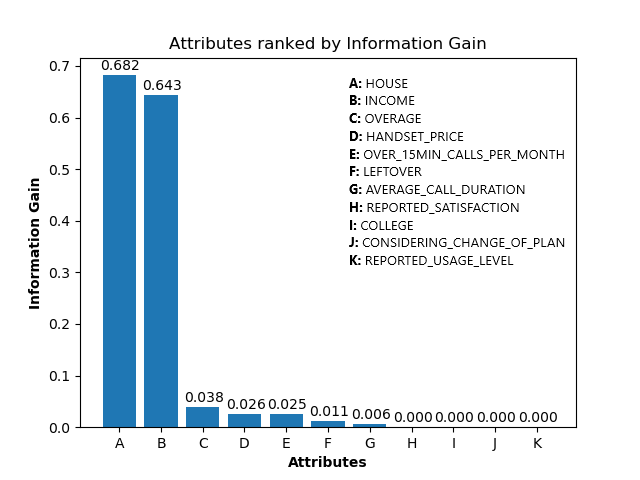
\includegraphics[scale=0.8]{InformationGain.png}
	\caption{Attributes ranked by their information gain}
	\centering 
	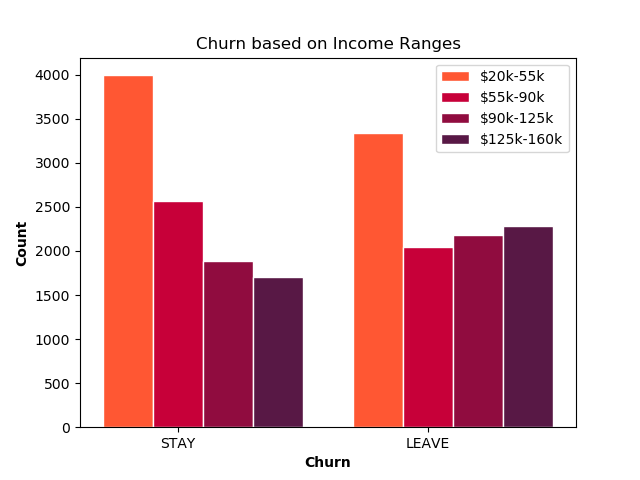
\includegraphics[scale=0.8]{IncomeVsChurn.png}
	\caption{Income vs Churn}
\end{figure}

\section{Customer Segmentation with $k$-means}
Before training a $k$-means model on the dataset, I first had to scale the data so that the magnitudes would not be so vastly different. To do this, I used the \texttt{StandardScaler} function from Python's \texttt{sklearn} module. I then used \texttt{sklearn}'s \texttt{KMeans} function for the $k$-means model along with the \texttt{k-means++} centroid initializer. \\\\
In order to determine the best value of $k$, I trained many different $k$-means models each with a different $k$ from $k=2 \rightarrow 25$. I then created two plots: a Sum Squared Error (SSE) plot and a Silhouette plot, \textbf{Figure 3} and \textbf{Figure 4}, respectively. I used the elbow method, along with the silhouette plot, to determine that a $k$-means model with $k=5$ would result in the optimal clustering.\\\\
The code for the $k$-means model and its analysis can be found in \texttt{../src/kmeans.py}.
\begin{figure}[H]
	\centering
	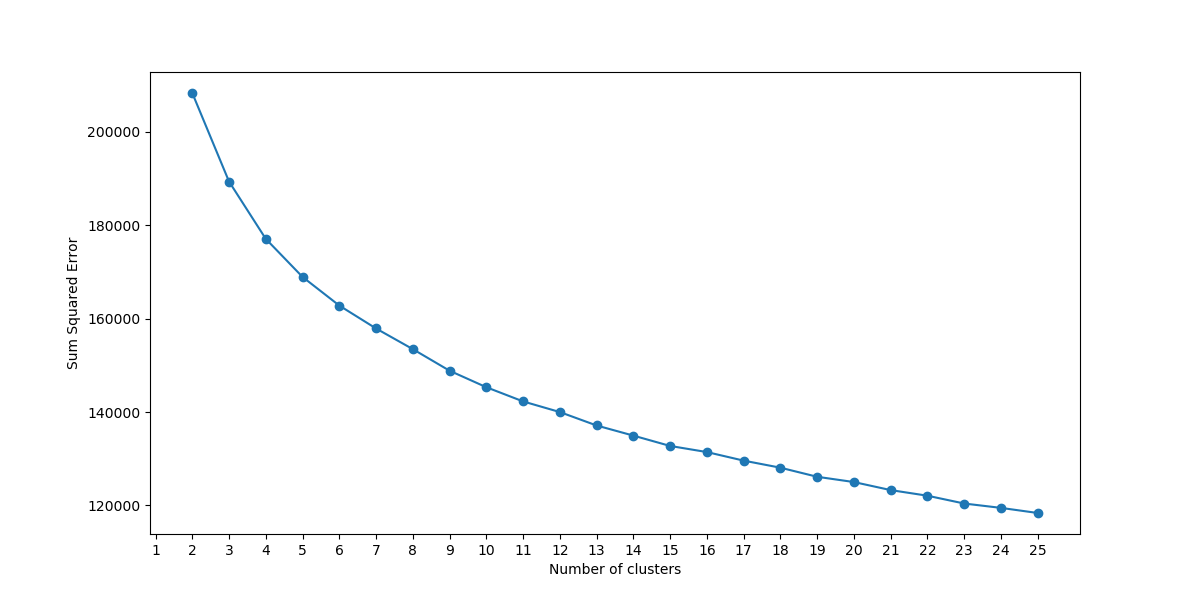
\includegraphics[scale=0.6]{kmeans_SSE.png}
	\caption{SSE plot}
	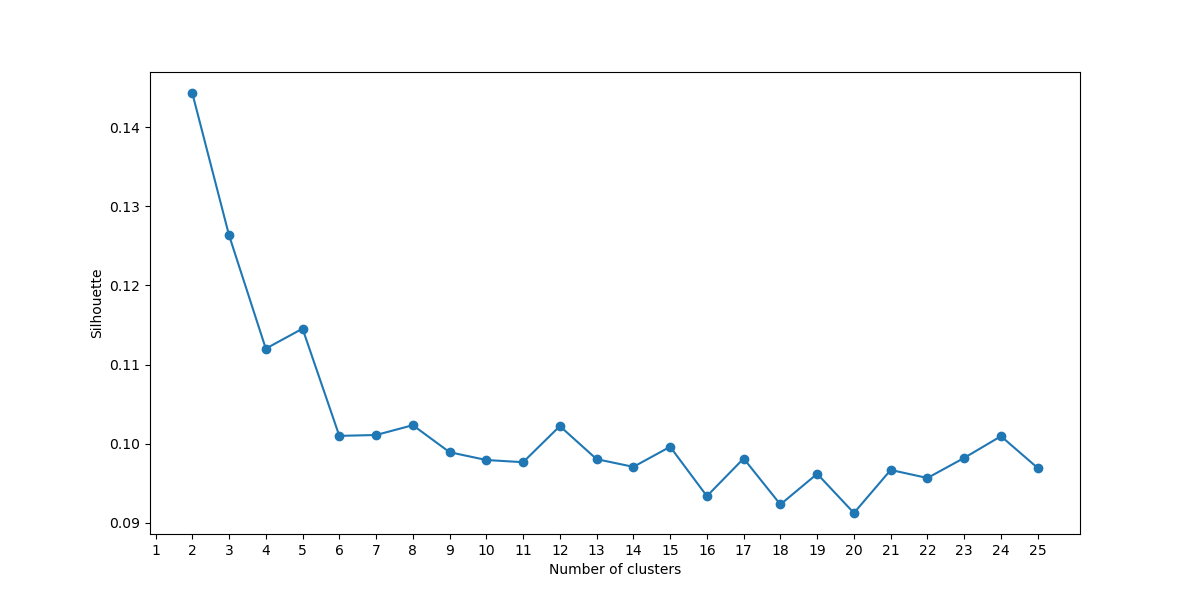
\includegraphics[scale=0.6]{kmeans_silhouette.png}
	\caption{Silhouette plot}
\end{figure}
\subsection{Cluster Analysis ($k=5$)}
The following tables contain the mean and standard deviation for each attribute and number of points in each of the 5 clusters. The raw data, which contains more information in the form of a five-number summary for each attribute (I did not include this due to space), can be found in \texttt{../data/cluster\_descriptions.txt}. One thing that I would like to note is that since many of the attributes were label encoded, the mean for such attributes would represent the average frequency of attribute values in the cluster. \\\\
From the tables, we can see that the attributes \texttt{College}, \texttt{House}, \texttt{Reported Satisfaction}, \texttt{Reported Usage Level}, and \texttt{Considering Change of Plan} had very little variation among the average values between clusters. This might signify that these attributes did not have much affect on the clustering process. \\\\
We can see that Cluster 1 had on average, higher \texttt{Income}, higher \texttt{Overage}, moderate \texttt{Leftover} minutes, higher \texttt{Handset Price}, higher number of \texttt{Over 15 Min Calls per Month}, and a higher number of "Leave" values for the \texttt{Leave} attribute. In contrast, Cluster 2 had on average, lower \texttt{Income}, lower \texttt{Overage}, lower \texttt{Leftover}, lower \texttt{Handset Price}, lower number of \texttt{Over 15 Min Calls per Month}, and a higher number of "Stay" values for the \texttt{Leave} attribute. Cluster 2 also has the most amount of points (6061 points), which shows that a large amount of the total points have lower than average values for their attributes.
\begin{table}[H]
	\centering
	\caption{Cluster 1 (2212 points)}
	\begin{tabular}{|l|l|l|l|l|l|l|l|}
		\cline{1-8}
		& College & Income & Overage & Leftover & House   & Handset Price & Over 15 Min Calls per Month \\
		\cline{1-8}
		Mean & 0.509 & 128118 &  193.77 & 24.25 &487948 &  641.66&  18.86\\
		\cline{1-8}
		Std  & 0.500&  22094 &   42.80  & 26.79 & 250777  & 159.40  &   6.85 \\
		\cline{1-8}
		\end{tabular}\\
		\begin{tabular}{|l|l|l|l|l|l|}
		\cline{1-6}
		& Avg Call Duration & Reported Satis. & Reported Usage Lvl. & Consid. Change Plan & Leave\\
		\cline{1-6}
		Mean & 6.014 & 1.540 & 1.784 & 2.506 & 0.823\\
		\cline{1-6}
		Std & 4.408 & 1.623 & 1.494 & 1.317 &  0.381\\
		\cline{1-6}
	\end{tabular}
\end{table}
\begin{table}[H]
	\centering
	\caption{Cluster 2 (6061 points)}
	\begin{tabular}{|l|l|l|l|l|l|l|l|}
		\cline{1-8}
		& College & Income & Overage & Leftover & House   & Handset Price & Over 15 Min Calls per Month \\
		\cline{1-8}
		Mean & 0.509  & 56155   & 32.07 &    7.64 & 495074 &  263.20 &    2.60\\
		\cline{1-8}
		Std  & 0.499 &  25797  &  39.57  &   9.76  &251585   & 94.22  &   3.13 \\
		\cline{1-8}
	\end{tabular}\\
	\begin{tabular}{|l|l|l|l|l|l|}
		\cline{1-6}
		& Avg Call Duration & Reported Satis. & Reported Usage Lvl. & Consid. Change Plan & Leave\\
		\cline{1-6}
		Mean & 8.176  &   1.572  &   1.834    & 2.430   &  0.326\\
		\cline{1-6}
		Std & 3.947 & 1.625 &  1.517  &   1.338   &  0.468\\
		\cline{1-6}
	\end{tabular}
\end{table}
\begin{table}[H]
	\centering
	\caption{Cluster 3 (3716 points)}
	\begin{tabular}{|l|l|l|l|l|l|l|l|}
		\cline{1-8}
		& College & Income & Overage & Leftover & House   & Handset Price & Over 15 Min Calls per Month \\
		\cline{1-8}
		Mean & 0.487 &  66323  &  45.67  &  60.66 &499972  & 305.00 &    3.52\\
		\cline{1-8}
		Std  &0.499  & 33610  &  56.78  &  18.82 & 254140 &  137.91  &   4.49 \\
		\cline{1-8}
	\end{tabular}\\
	\begin{tabular}{|l|l|l|l|l|l|}
		\cline{1-6}
		& Avg Call Duration & Reported Satis. & Reported Usage Lvl. & Consid. Change Plan & Leave\\
		\cline{1-6}
		Mean & 1.786  &   1.581  &   1.797   &  2.527   &  0.511\\
		\cline{1-6}
		Std & 1.424 & 1.625  &1.514 &  1.301 & 0.499\\
		\cline{1-6}
	\end{tabular}
\end{table}
\begin{table}[H]
	\centering
	\caption{Cluster 4 (4106 points)}
	\begin{tabular}{|l|l|l|l|l|l|l|l|}
		\cline{1-8}
		& College & Income & Overage & Leftover & House   & Handset Price & Over 15 Min Calls per Month \\
		\cline{1-8}
		Mean & 0.491 &  56220 &  195.48  &  19.85&  489171  & 263.13  &  19.29\\
		\cline{1-8}
		Std  & 0.499 &  25241  &  40.70   & 23.47 & 252382  &  93.23 &    6.48 \\
		\cline{1-8}
	\end{tabular}\\
	\begin{tabular}{|l|l|l|l|l|l|}
		\cline{1-6}
		& Avg Call Duration & Reported Satis. & Reported Usage Lvl. & Consid. Change Plan & Leave\\
		\cline{1-6}
		Mean &6.268 &  1.519 &   1.811 &  2.552 &   0.597\\
		\cline{1-6}
		Std & 4.321 &   1.627 &   1.513 &    1.314  &   0.490\\
		\cline{1-6}
	\end{tabular}
\end{table}
\begin{table}[H]
	\centering
	\caption{Cluster 5 (3905 points)}
	\begin{tabular}{|l|l|l|l|l|l|l|l|}
		\cline{1-8}
		& College & Income & Overage & Leftover & House   & Handset Price & Over 15 Min Calls per Month \\
		\cline{1-8}
		Mean & 0.513 & 129211  &  31.79  &  18.18 & 490828 &  656.55  &   2.59\\
		\cline{1-8}
		Std  & 0.499  & 21348 &   37.56 &   21.58 & 252931   &151.90   &  2.88 \\
		\cline{1-8}
	\end{tabular}\\
	\begin{tabular}{|l|l|l|l|l|l|}
		\cline{1-6}
		& Avg Call Duration & Reported Satis. & Reported Usage Lvl. & Consid. Change Plan & Leave\\
		\cline{1-6}
		Mean & 6.352  &   1.604  &   1.824   &  2.492  &   0.434\\
		\cline{1-6}
		Std & 4.251  &   1.643   &  1.509  &   1.329  &  0.495\\
		\cline{1-6}
	\end{tabular}
\end{table}

\section{Predictive Models}
\subsection{Decision Trees}
The first type of predictive model I chose was the decision tree classifier. The decision tree model I used was \texttt{sklearn}'s \texttt{DecisionTreeClassifier} function. The hyper-parameters I tuned were: Gini impurity to measure the quality of a split and a max tree depth of 10. This model was trained and tested with a 75/25 split on the dataset, with 75\% of the dataset used for the training data. The decision tree classifier had on average 68\% accuracy on the test data.\\\\
In an attempt to improve my testing accuracy, I decided to implement the random forest model, which is an ensemble learning method that improves upon the decision tree method by correcting their habit of over-fitting. Random forests do this by constructing a multitude of decision trees at training time and outputting the class that is the mode of the classes. The random forest model I used was \texttt{sklearn}'s \texttt{RandomForestClassifier} function. Using the same data split as the decision tree classifier, my random forest model saw little improvement; the model had on average an accuracy of 70\%. \\\\
The code for these models can be found in \texttt{../src/decisiontree.py}.
\subsection{Neural Network}
The next type of predictive model I chose was a simple feed-forward neural network. The model I used was a \texttt{keras} \texttt{Sequential} model. Like the decision tree model, I trained and validated the neural network using a 75/25 training and test split of the dataset. I created three different models, each with different hidden layer dimensions: \textbf{Figure 5:} 11x32x16x4x1, \textbf{Figure 6:} 11x64x32x16x4x1, and \textbf{Figure 7:} 11x128x64x32x16x8x4x1. The first layer in each model is 11 nodes for the 11 attributes, and the output layer is 1 node for the \texttt{Leave} attribute. All of my models trained on 20 epochs, used the binary cross-entropy loss function, and used the ReLU activation function on all layers except for the output layer, which used the sigmoid function.  \\\\
The models had testing accuracies of 68.15\%, 68.18\%, and 67.78\% for figures 5, 6, and 7, respectively. The difference in accuracies is basically negligible, so we can see that the change in model dimensions doesn't affect the performance for this specific dataset. These also may not be the best hyper-parameters, so the model performance could be better. \\\\
The code for the neural network model can be found in \texttt{../src/neuralnet.py}.

\begin{figure}[H]
	\centering
	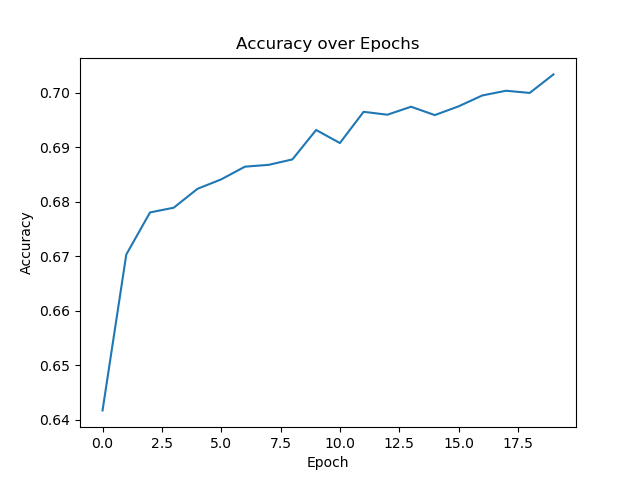
\includegraphics[scale=0.6]{neuralnet1.png}
	\caption{Dimensions: 11x32x16x4x1, Test Accuracy: 68.15\%}
\end{figure}
\begin{figure}[H]
	\centering
	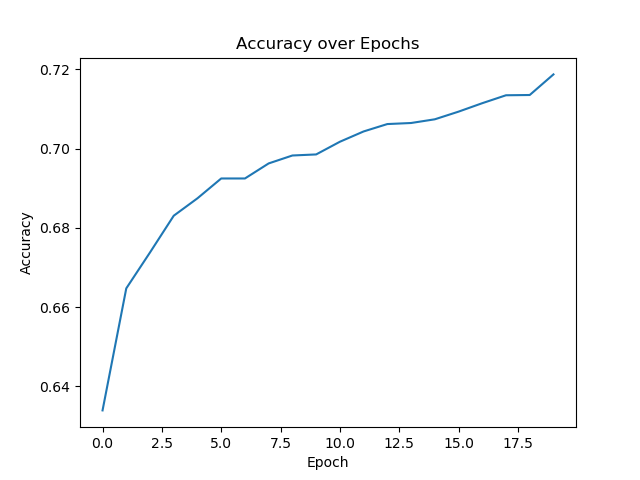
\includegraphics[scale=0.6]{neuralnet2.png}
	\caption{Dimensions: 11x64x32x16x4x1, Test Accuracy: 68.18\%}
\end{figure}
\begin{figure}[H]
	\centering
	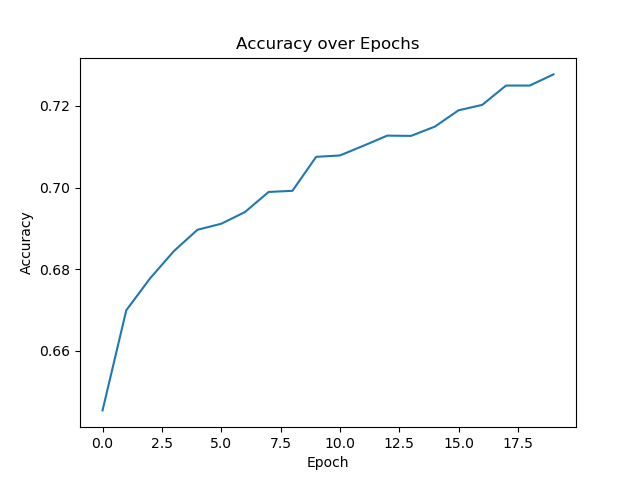
\includegraphics[scale=0.6]{neuralnet3.png}
	\caption{Dimensions: 11x128x64x32x16x8x4x1, Test Accuracy: 67.78\%}
\end{figure}

\section{Analysis}
Both the decision tree model and the neural network model achieved testing accuracies of about 68\%. The random forest model, which was done to try and improve upon the decision tree model, achieved slightly better results, with a testing accuracy of 70\$. All of these models were trained using 75\% of the dataset, and tested on the remaining 25\%. The data was shuffled before being split to try and mitigate any hidden patterns in the data ordering. \\\\
In general, the data was balanced; upon analysis of the values under the \texttt{Leave} attribute, there were 10,148 entries under the "STAY" class, and 9,853 entries under the "LEAVE" class. Since the data seems balanced, I don't have to worry about the impacts of un-balanced data on my model performance.\\\\


\end{document}